% -*- mode:LaTex; mode:visual-line; mode:flyspell; fill-column:75-*-

\chapter{Introduction} \label{secIntro}

% Introduction.

% \section{Installation instructions}

% This template was tested with TeX Live 2017, which includes all required packages~\cite{TUG2017}. Mac users: this is included as part of OSX and TeXShop. After successfully installing TeX Live, compile the PDF file using your favorite build tool (we tested with \verb!make! on OSX).

% \section{How to use this template}
% Write each chapter as a separate \LaTeX\ file and include them in \verb!thesis-main.tex!. Edit the abstract, acknowledgments, background, title, dedication, and funding files as necessary. Include additional packages in \verb!thesis-packages.tex! and define helpful macros in \verb!thesis-macros.tex!.

% \subsection{Algorithms}
% Define each algorithm as a separate \LaTeX\ file in the algorithms folder using either the \verb!algorithmicx! or \verb!algpseudocode! packages. For example, see Algorithm~\ref{algTemplate}.

% \input{algorithms/alg-template.tex}
\section{SLAM}

Simultaneous Localization and Mapping (SLAM) is the chicken-and-egg problem of estimating the environment represented as a map, and simultaneously optimizing the robot trajectory associated with the map, given measurements.

Typically, when the map is modeled as a collection of landmarks $ \Lc = \{\ell_m\}_{m=1}^{M} $, and the robot trajectory is modeled as a sequence of poses $\Xc = \{\xv_t\}_{t=1}^{T}$, given a set of measurements $ \Zc = \{\zv_n\}_{n=1}^{N}$, the SLAM problem can be summarized as a maximum-a-posteriori estimation \cite{dellaertFactorGraphsRobot2017} as follows:
\begin{align}
    \hat{\Xc}, \hat{\Lc} &= \argmax_{\Xc, \Lc} p(\Xc, \Lc | \Zc) \\
                         &\propto \argmax_{\Xc, \Lc} p(\Zc | \Xc, \Lc) p(\Xc, \Lc)
\end{align}
Note, that the above problem assumes known \emph{data association} between measurements $\zv_n$ of landmark $\ell_{\beta_n}$ at a robot pose $\xv_{\alpha_n}$as $\Dc := \{(\alpha_n, \beta_n)\}_{n=1}^{N}$ \cite{bowmanProbabilisticDataAssociation2017}.

In reality, however, a SLAM framework for a robot needs to deal with raw sensor measurements. Therefore, typically the system is divided into two parts: \emph{front-end} and \emph{back-end}. The front-end is dedicated to data pre-processing, data association and feeds into the back-end dedicated to the optimization that results in the best estimate of robot state and landmarks.

\section{Semantics in SLAM}

For autonomous robots in the near future to work in the real world, advanced interpretation of the environment is necessar. For workloads ranging from semantic 3D reconstruction and path planning, to active interaction with the environment (see Figure~\todo{Add figure of household robot}). These workloads require not only geometric perception including robot localization and map reconstruction, but also semantic and compositional understanding of scenes.

In recent years, geometry-based SLAM has achieved high levels of performance in \textit{experimental setups} for localization tasks. Many variants of SLAM algorithms, from ORB-SLAM~\cite{mur-artalORBSLAM2OpenSourceSLAM2017} to Direct Sparse Odometry (DSO)~\cite{engelDirectSparseOdometry2018}, can now run in real-time with high trajectory accuracy.
However, they are in general limited by the \emph{static-world} assumption and low-level scene representation as sparse 3D feature points, and thus cannot distill high-level information (semantic understanding) in scenes and adjust to structured environmental changes.

On the other hand, with progress in deep learning, near real-time semantic perception is achievable powered by efficient Deep Neural Networks (DNNs).
Researchers have started to switch to semantic SLAM taking advantage of off-the-shelf solutions; pioneering research includes SLAM++~\cite{salas-morenoSLAMSimultaneousLocalisation2013}, Fusion++~\cite{mccormacFusionVolumetricObjectLevel2018}, and MaskFusion~\cite{runzMaskFusionRealTimeRecognition2018}. These initial attempts take into consideration semantic segmentation, but typically simply attach DNN frontends to existing SLAM frameworks in an ad hoc fashion. Implementation-wise, they require high-end machines to achieve near real-time performance, or are not available to the community.

\section{Contributions}

\begin{enumerate}
    \item A compositional volumetric rendering method that selects objects of interest and reduces memory footprint;
    \item A hybrid object association method that combines geometric and semantic cues to enable drift-free tracking without an explicit relocalization module;
    \item A scalable, modular, and easy-to-use open source system that runs nearly realtime.
\end{enumerate}
%While there exist many Simultaneous Localization and Mapping (SLAM) systems that utilize geometric consistencies for scene reconstruction and robot state estimation, we only see adoption of these systems for low level tasks such as visualization, occupancy prediction, and inspection. Enabling practical use of SLAM for higher level tasks requires that the robot has a geometric as well as a semantic understanding of its environment.

To address these problems, we propose a novel modular solution that concentrates on recognizable persistent object landmarks. In theory, we derived a compositional and scalable object map for robust tracking. In implementation, we fully exploit the power of the modern GPU-based reconstruction pipeline~\cite{dong2019gpu} and object detection frameworks ~\cite{kirillov_pointrend_2020}, to design an efficient architecture for data exchange without sacrificing the ease of system configuration and build.

% In addition to a classical SLAM framework that focuses on the MAP estimation of the sequence of agent poses and the landmark positions, the Object SLAM framework typically incorporates a 2D object detector (such as Mask-RCNN or YOLO-V3), that outputs bounding boxes or masks of potential objects. This generalizes the SLAM problem to a joint maximum likelihood estimation of data association between landmarks, the landmark position, and the sequence of agent poses [2].

% High-fidelity reconstruction of indoor environments is an interesting but challenging problem. Successful reconstruction can enable new applications in robotics, particularly in the human-robot interaction space. Building object-oriented maps that combine semantic and geometric information of the environment will help robots interact with the complex dynamics of household and industrial deployment scenarios with greater ease. Our work proposes an online object level semantic map representation that can enable online tracking of low dynamic objects, and simultaneously provide improved accuracy of the map. Moreover, this work also proposes a method of loop-closure using divergence to quantify the association/similarity between two sets of captured data.

\begin{figure}[t!]
    \centering
    \includegraphics[width=\linewidth]{figs/teaser.pdf}\vspace{-1cm}
%    \includegraphics[width=\linewidth]{figures/scene14.png}
    \caption{Reconstruction of \textit{fr2\_xyz} sequence from \emph{tum rgbd} dataset. Our pipeline can reconstruct both camera trajectory and object models in the scene.}
    \label{fig:objectsandscene}
\end{figure}

Our main contributions in this paper are:



 \begin{figure*}[ht!]
 	\centering
    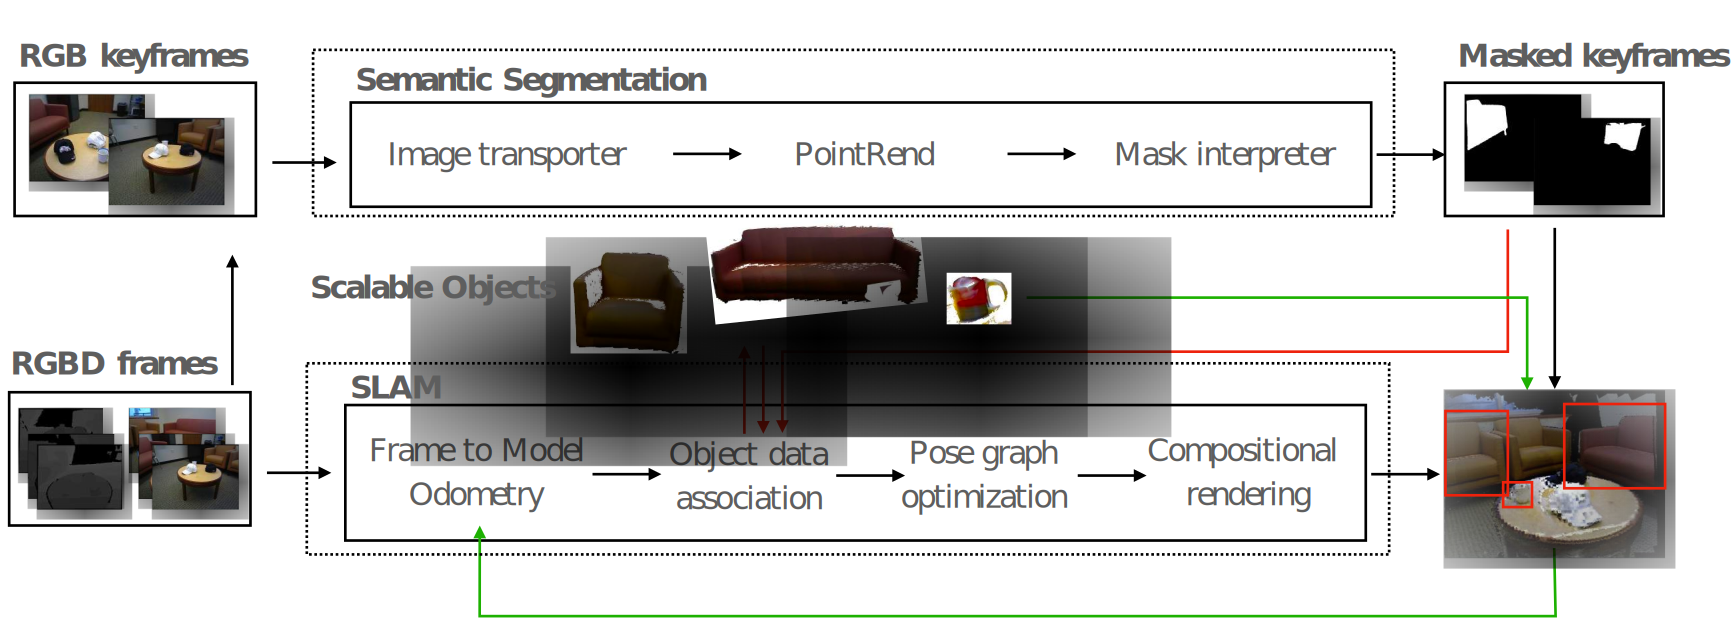
\includegraphics[width=0.90\linewidth]{figs/icra2021-compressed.pdf}
    \caption{\label{fig:overview} System overview: Top shows the deep object segmentation pipeline that runs asynchronously, Masked keyframes from the segmentation pipeline are used in Data association and map update (shown with red lines). Bottom shows the major stages of the reconstruction system, specifically object models are used in tracking via compositional raycasting (shown with green lines).}
    \vspace*{-1em}
 \end{figure*}

%Introduction shall mainly start from and would cover the following topics:
%\begin{enumerate}
%	\item Motivation of the problem
%	\item What are the general ways the problem is solved currently?
%	\item  Shortcomings of the current state-of-the-art or the one with whom I am comparing against
%	\item Proposed approach bridging that gap somehow? Cite Fig.~\ref{fig:glory_shot} here.
%	\item Core contributions enumeration
%	\item Paper structure
%\end{enumerate}


%%% Local Variables:
%%% mode: latex
%%% TeX-master: "main"
%%% End:
